% Chapter Template
\chapter{4 Tensor Decomposition} % Main chapter title
\label{Chapter4}
\def \path	{Figures/C4}
In questo capitolo verranno messi in pratica i concetti introdotti nel Capitolo \ref{Capitolo3}. In particolare, verrà addestrata una CNN su 2 dataset, MNIST e CIFAR. I risultati su quest'ultimo serviranno da confronto con ResNet, la rete utilizzata nel Capitolo 5. 
%--------------------------------------------------------------------
%	SECTION 1
%--------------------------------------------------------------------
\section{Background}}
%% intro 

%% SVD Applied on Fully Connected layer 

$$ (U_{n \times t}\Sigma_{t \times t}V^T_{m \times t})x + b $$ = $$ U_{n \times t} ( \Sigma_{t \times t}V^T_{m \times t} x ) + b $$


%--------------------------------------------------------------------
%	SECTION 2
%--------------------------------------------------------------------
\section{}


%--------------------------------------------------------------------
%	SECTION 3
%--------------------------------------------------------------------
\section{MNIST: preprocessing}


%%inserire codice per dataset MNIST %% 
%--------------------------------------------------------------------
%	SECTION 4
%--------------------------------------------------------------------
\section{MNIST: addestramento}


%--------------------------------------------------------------------
%	SECTION 5
%--------------------------------------------------------------------
\section{CIFAR: preprocessing}




%--------------------------------------------------------------------
%	SECTION 6
%--------------------------------------------------------------------
\section{CIFAR: addestramento}




%%%%%%%%%%%%%%%%%%%%%%%%%%%%%%%%%%%%%%%%%%%%%%%%%%
%%%%%%%%%%%%%%%%%%%%%%%%%%%%%%%%%%%%%%%%%%%%%%%%%%

%% Approximation with CPD 

\begin{equation}
$$ \sum_{r=1}^R K^x_r(i)K^y_r(j)K^s_r(s)K^t_r(t) $$.	
\end{equation}


%%%% forward pass con CPD %%% 
\begin{center}
\begin{align*}
	V(x, y, t) = \sum_i \sum_j \sum_s K(x-i, y-j, s, t)X(i, j, s) \\
		= \sum_r \sum_i \sum_j \sum_s K^x_r(x-i)K^y_r(y-i)K^s_r(s)K^t_r(t)X(i, j, s)\\
			= \sum_r K^t_r(t) \sum_i \sum_j K^x_r(x-i)K^y_r(y-i) \sum_s K^s_r(s) X(i, j, s) \tag{4}
\end{align*}
\end{center}


%% forward pass con Tucker 
The Tucker decomposition, also known as the Higher Order SVD  \emph{HOSVD} is a generalization of SVD for tensors: 

$$ K(i, j, s, t) = \sum_{r_1=1}^{R_1}\sum_{r_2=1}^{R_2}\sum_{r_3=1}^{R_3}\sum_{r_4=1}^{R_4}G_{r_1, r_2, r_3, r_4} * K^x_{r1}(i)K^y_{r2}(j)K^s_{r3}(s)K^t_{r4}(t) $$

The Tucker decomposition has a property that's useful for our purposes: it doesn't have to be applied along all modes (axis) of the tensors. We have seen how CPD decomposes the kernel also spatial-wise; this acts
pretty aggressively on the number of parameters and since the convolutional kernels are small in most of the recent implementations ($3x3$ or $5x5$) it arguably doesn't save a lot of computation. Hence, we can skip
this decomposition with Tucker, going for what is known as a Tucker-2 decomposition: 

\begin{equation}
\label{eq:tucker-def}
	K(i, j, s, t) = \sum_{r_3=1}^{R_3}\sum_{r_4=1}^{R_4} \textbf{G} {i,j,r_3, r_4}(j)K^s_{r3}(s)K^t_{r4}(t) 
\end{equation} 

Using equation \ref{eq:tucker-def} and plugging into the formula for the convolutional forward pass, we obtain the new equation for the Tucker convolutional forward pass: 

$$ V(x, y, t) = \sum_i \sum_j \sum_sK(x-i, y-j, s, t)X(i, j, s) $$

$$ V(x, y, t) = \sum_i \sum_j \sum_s\sum_{r_3=1}^{R_3}\sum_{r_4=1}^{R_4}\sigma_{(x-i)(y-j) r_3 r_4}K^s_{r3}(s)K^t_{r4}(t)X(i, j, s) $$

$$ V(x, y, t) = \sum_i \sum_j \sum_{r_4=1}^{R_4}\sum_{r_3=1}^{R_3}K^t_{r4}(t)\sigma_{(x-i)(y-j) r_3 r_4} \sum_s\ K^s_{r3}(s)X(i, j, s) $$ 



\begin{lstlisting}[language={[5.2]Lua}]
----- preprocess/normalize train/test sets -----
print '<trainer> preprocessing data (color space + normalization)'

-- preprocess trainSet
normalization = nn.SpatialContrastiveNormalization(1, image.gaussian1D(7))
for i = 1,trainData:size() do
   --rgb -> yuv
   local rgb = trainData.data[i]
   local yuv = image.rgb2yuv(rgb)
   
   -- normalize Y locally:
   yuv[1] = normalization(yuv[{{1}}])
   trainData.data[i] = yuv
end
-- normalize U globally:
mean_u = trainData.data[{ {},2,{},{} }]:mean()
std_u = trainData.data[{ {},2,{},{} }]:std()
trainData.data[{ {},2,{},{} }]:add(-mean_u)
trainData.data[{ {},2,{},{} }]:div(-std_u)

-- normalize V globally:
mean_v = trainData.data[{ {},3,{},{} }]:mean()
std_v = trainData.data[{ {},3,{},{} }]:std()
trainData.data[{ {},3,{},{} }]:add(-mean_v)
trainData.data[{ {},3,{},{} }]:div(-std_v)

--same applies to test set...
\end{lstlisting}



\begin{figure}[h!]
 \centering
 \includegraphics[width=1.0\textwidth]{\path/k-mode.png} 
  \caption{Example of k-mode multiplication on 3-dimensional tensor.}
 \label{fig:k-mode}
\end{figure}

\bigskip

\begin{figure}
\centering
\begin{subfigure}{.5\textwidth}
  \centering
 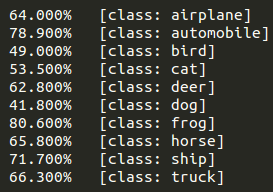
\includegraphics[width=1\textwidth]{\path/cifar-tanh.png} 
  \caption{Acc.= \textasciitilde 65\% f. di attivazione = TanH}
 \label{fig:training}
\end{subfigure}%
\begin{subfigure}{.5\textwidth}
  \centering
 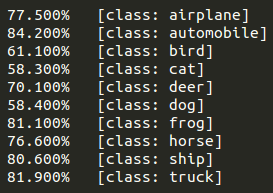
\includegraphics[width=1\textwidth]{\path/cifar-relu.png} 
  \caption{Acc.= \textasciitilde 73\% f. di attivazione = ReLU}
 \label{fig:validation}
\end{subfigure}
\caption{Percentuali di accuracy a seconda della funzione d'attivazione. La ReLU produce indubbiamente risultati migliori.}
\label{fig:relu}
\end{figure}
\\
%%%%% NEW PAGE FOR THE NEW FIGURES %%%% 
\newpage
\pagebreak
\medskip
\newpage

\begin{figure}[h!]
 \centering
 \includegraphics[width=1.0\textwidth]{\path/tensor-mode.jpg} 
 \caption{Fibers and slices of a tensor: fibers is an equivalent term for a tensor mode.}
 \label{fig:tensor-fibers}
\end{figure}

\begin{figure}[h!]
 \centering
 \includegraphics[width=1.0\textwidth]{\path/tucker-pass.jpg} 
 \caption{Tucker-2  decompositions  for  speeding-up  a generalized convolution. Each box corresponds to a 3-way tensor $X, Z, Z^' and Y$ in equation (\ref{eq:tucker1}-\ref{eq:tucker3}). Arrows represent linear mappings 
and illustrate each scalar value on the right is computed. Red tube, green cube and blue tube correspond to 
1x1, dxd and 1x1 convolution respectively.}
 \label{fig:tucker-pass}
\end{figure}


\begin{figure}[h!]
 \centering
 \includegraphics[width=1.0\textwidth]{\path/CPD.jpg} 
 \caption{Tensor decompositions for speeding up a generalized convolution. Each box correspond to a feature map stack within a CNN, (frontal sides are spatial dimensions). Arrows show linear mappings and demonstrate how scalar values on the right are computed. Initial full convolution (A) computes each element of the target tensor as a linear combination of the elements of a 3D subtensor that spans a spatial d × d window over all input maps. 
Jaderberg et al. (B) approximate the initial convolution as a composition of two linear mappings in which the intermediate mpa stack has R  maps, being R the rank of the decomposition. Each of the two-components 
computes each target value with a convolution based on a spatial window of size dx1 or 1xd in all input maps. Finally, CP-decomposition (C) by Lebedev et al. approximates the convolution as a composition of four smaller convolutions: the first and the last components compute a standard 1x1 convolution that spans all input maps while the middle ones compute a 1D grouped convolution \textbf{only on one} input map.}
 \label{fig:cpd-pass}
\end{figure}

Tensor decompositions for speeding up a generalized convolution. Gray boxes corre-
spond to 3D tensors (map stacks) within a CNN, with the two frontal sides corresponding to spatial
dimensions. Arrows show linear mappings and demonstrate how scalar values on the right (small
boxes corresponding to single elements of the target tensor) are computed. Initial full convolu-
tion (a) computes each element of the target tensor as a linear combination of the elements of a
3D subtensor that spans a spatial d × d window over all input maps. Jaderberg et al. (2014a) (b)
approximate the initial convolution as a composition of two linear mappings with the intermediate
map stack having R maps (where R is the rank of the decomposition). Each of the two mappings
computes each target value based on a spatial window of size 1×d or d×1 in all input maps. Finally,
CP-decomposition (c) used in our approach approximates the convolution as a composition of four
convolutions with small kernels, so that a target value is computed based on a 1D-array that spans
either one pixel in all input maps, or a 1D spatial window in one input map.
\\

